% GNUPLOT: LaTeX picture with Postscript
\begingroup
  \makeatletter
  \providecommand\color[2][]{%
    \GenericError{(gnuplot) \space\space\space\@spaces}{%
      Package color not loaded in conjunction with
      terminal option `colourtext'%
    }{See the gnuplot documentation for explanation.%
    }{Either use 'blacktext' in gnuplot or load the package
      color.sty in LaTeX.}%
    \renewcommand\color[2][]{}%
  }%
  \providecommand\includegraphics[2][]{%
    \GenericError{(gnuplot) \space\space\space\@spaces}{%
      Package graphicx or graphics not loaded%
    }{See the gnuplot documentation for explanation.%
    }{The gnuplot epslatex terminal needs graphicx.sty or graphics.sty.}%
    \renewcommand\includegraphics[2][]{}%
  }%
  \providecommand\rotatebox[2]{#2}%
  \@ifundefined{ifGPcolor}{%
    \newif\ifGPcolor
    \GPcolortrue
  }{}%
  \@ifundefined{ifGPblacktext}{%
    \newif\ifGPblacktext
    \GPblacktexttrue
  }{}%
  % define a \g@addto@macro without @ in the name:
  \let\gplgaddtomacro\g@addto@macro
  % define empty templates for all commands taking text:
  \gdef\gplbacktext{}%
  \gdef\gplfronttext{}%
  \makeatother
  \ifGPblacktext
    % no textcolor at all
    \def\colorrgb#1{}%
    \def\colorgray#1{}%
  \else
    % gray or color?
    \ifGPcolor
      \def\colorrgb#1{\color[rgb]{#1}}%
      \def\colorgray#1{\color[gray]{#1}}%
      \expandafter\def\csname LTw\endcsname{\color{white}}%
      \expandafter\def\csname LTb\endcsname{\color{black}}%
      \expandafter\def\csname LTa\endcsname{\color{black}}%
      \expandafter\def\csname LT0\endcsname{\color[rgb]{1,0,0}}%
      \expandafter\def\csname LT1\endcsname{\color[rgb]{0,1,0}}%
      \expandafter\def\csname LT2\endcsname{\color[rgb]{0,0,1}}%
      \expandafter\def\csname LT3\endcsname{\color[rgb]{1,0,1}}%
      \expandafter\def\csname LT4\endcsname{\color[rgb]{0,1,1}}%
      \expandafter\def\csname LT5\endcsname{\color[rgb]{1,1,0}}%
      \expandafter\def\csname LT6\endcsname{\color[rgb]{0,0,0}}%
      \expandafter\def\csname LT7\endcsname{\color[rgb]{1,0.3,0}}%
      \expandafter\def\csname LT8\endcsname{\color[rgb]{0.5,0.5,0.5}}%
    \else
      % gray
      \def\colorrgb#1{\color{black}}%
      \def\colorgray#1{\color[gray]{#1}}%
      \expandafter\def\csname LTw\endcsname{\color{white}}%
      \expandafter\def\csname LTb\endcsname{\color{black}}%
      \expandafter\def\csname LTa\endcsname{\color{black}}%
      \expandafter\def\csname LT0\endcsname{\color{black}}%
      \expandafter\def\csname LT1\endcsname{\color{black}}%
      \expandafter\def\csname LT2\endcsname{\color{black}}%
      \expandafter\def\csname LT3\endcsname{\color{black}}%
      \expandafter\def\csname LT4\endcsname{\color{black}}%
      \expandafter\def\csname LT5\endcsname{\color{black}}%
      \expandafter\def\csname LT6\endcsname{\color{black}}%
      \expandafter\def\csname LT7\endcsname{\color{black}}%
      \expandafter\def\csname LT8\endcsname{\color{black}}%
    \fi
  \fi
    \setlength{\unitlength}{0.0500bp}%
    \ifx\gptboxheight\undefined%
      \newlength{\gptboxheight}%
      \newlength{\gptboxwidth}%
      \newsavebox{\gptboxtext}%
    \fi%
    \setlength{\fboxrule}{0.5pt}%
    \setlength{\fboxsep}{1pt}%
\begin{picture}(7920.00,4800.00)%
    \gplgaddtomacro\gplbacktext{%
      \colorrgb{0.00,0.00,0.00}%
      \put(595,715){\makebox(0,0)[r]{\strut{}-40}}%
      \colorrgb{0.00,0.00,0.00}%
      \put(595,1366){\makebox(0,0)[r]{\strut{}-20}}%
      \colorrgb{0.00,0.00,0.00}%
      \put(595,2018){\makebox(0,0)[r]{\strut{} 0}}%
      \colorrgb{0.00,0.00,0.00}%
      \put(595,2669){\makebox(0,0)[r]{\strut{} 20}}%
      \colorrgb{0.00,0.00,0.00}%
      \put(595,3320){\makebox(0,0)[r]{\strut{} 40}}%
      \colorrgb{0.00,0.00,0.00}%
      \put(595,3972){\makebox(0,0)[r]{\strut{} 60}}%
      \colorrgb{0.00,0.00,0.00}%
      \put(595,4623){\makebox(0,0)[r]{\strut{} 80}}%
      \colorrgb{0.00,0.00,0.00}%
      \put(762,437){\makebox(0,0){\strut{}$0$}}%
      \colorrgb{0.00,0.00,0.00}%
      \put(1441,437){\makebox(0,0){\strut{}$20$}}%
      \colorrgb{0.00,0.00,0.00}%
      \put(2121,437){\makebox(0,0){\strut{}$40$}}%
      \colorrgb{0.00,0.00,0.00}%
      \put(2800,437){\makebox(0,0){\strut{}$60$}}%
      \colorrgb{0.00,0.00,0.00}%
      \put(3480,437){\makebox(0,0){\strut{}$80$}}%
      \colorrgb{0.00,0.00,0.00}%
      \put(4159,437){\makebox(0,0){\strut{}$100$}}%
      \colorrgb{0.00,0.00,0.00}%
      \put(4838,437){\makebox(0,0){\strut{}$120$}}%
      \colorrgb{0.00,0.00,0.00}%
      \put(5518,437){\makebox(0,0){\strut{}$140$}}%
      \colorrgb{0.00,0.00,0.00}%
      \put(6197,437){\makebox(0,0){\strut{}$160$}}%
      \colorrgb{0.00,0.00,0.00}%
      \put(6877,437){\makebox(0,0){\strut{}$180$}}%
      \colorrgb{0.00,0.00,0.00}%
      \put(7556,437){\makebox(0,0){\strut{}$200$}}%
    }%
    \gplgaddtomacro\gplfronttext{%
      \csname LTb\endcsname%
      \put(143,2669){\rotatebox{-270}{\makebox(0,0){\strut{}$i\ped{dc}(t), i\ped{ac}(t), i(t) \, / \si{kA}$}}}%
      \csname LTb\endcsname%
      \put(7753,2669){\rotatebox{-270}{\makebox(0,0){\strut{}}}}%
      \csname LTb\endcsname%
      \put(4159,139){\makebox(0,0){\strut{}$t / \si{ms}$}}%
      \csname LTb\endcsname%
      \put(4159,4524){\makebox(0,0){\strut{}}}%
      \csname LTb\endcsname%
      \put(4159,4523){\makebox(0,0){\strut{}}}%
      \csname LTb\endcsname%
      \put(243,100){\makebox(0,0)[l]{\strut{}}}%
      \csname LTb\endcsname%
      \put(6944,4395){\makebox(0,0){\strut{}}}%
      \csname LTb\endcsname%
      \put(6852,4320){\makebox(0,0)[l]{\strut{}$i\ped{dc}(t)$}}%
      \csname LTb\endcsname%
      \put(6852,4022){\makebox(0,0)[l]{\strut{}$i\ped{ac}(t)$}}%
      \csname LTb\endcsname%
      \put(6852,3724){\makebox(0,0)[l]{\strut{}$i(t)$}}%
    }%
    \gplbacktext
    \put(0,0){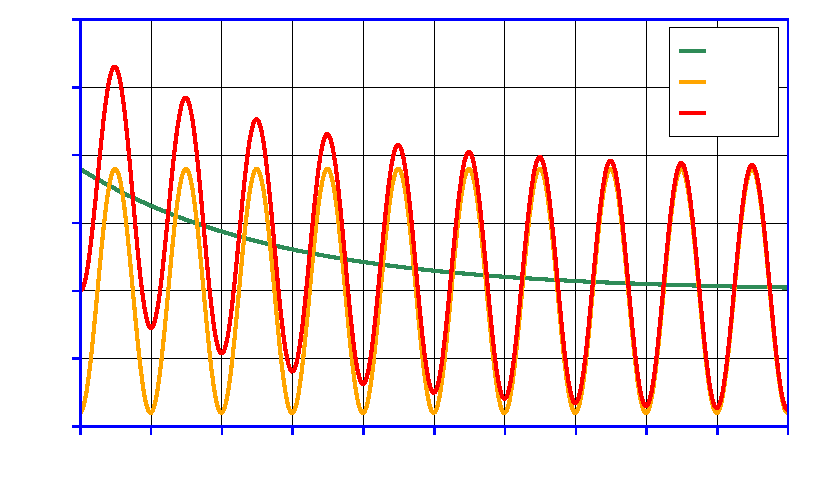
\includegraphics{Cap-Fonaments-RL-Serie-Curtcircuit-Exemple}}%
    \gplfronttext
  \end{picture}%
\endgroup
